\section{Il modello multidimensionale}

È il modello utilizzato per la rappresentazione delle informazioni all’interno dei data mart. Si è scelto questo modello perché molto intuitivo ed è già alla base del foglio elettronico che i manager sono abituati ad utilizzare. L’altro motivo per cui è stato  scelto è che larga parte delle query OLAP sono facilmente formulabili proprio in riferimento al modello multidimensionale. Il punto fondamentale è il concetto di \textbf{fatto}, ovvero un fenomeno di business che accade dinamicamente nell’azienda e che gli utenti sono interessati a monitorare (vendita, spedizione, fattura). In una prima presentazione del modello multidimensionale si usa una metafora che è quella del cubo, fatto da tante celle e costituito da tre spigoli, che rappresentano le dimensioni, ovvero attributi che sono utilizzati per selezionare e aggregare le celle dei cubi. Dentro ad una cella vi è un numero, che noi chiamiamo \textbf{misura}, il quale quantifica il fatto da un certo punto di vista. 
\begin{figure}[H]
	\centering
	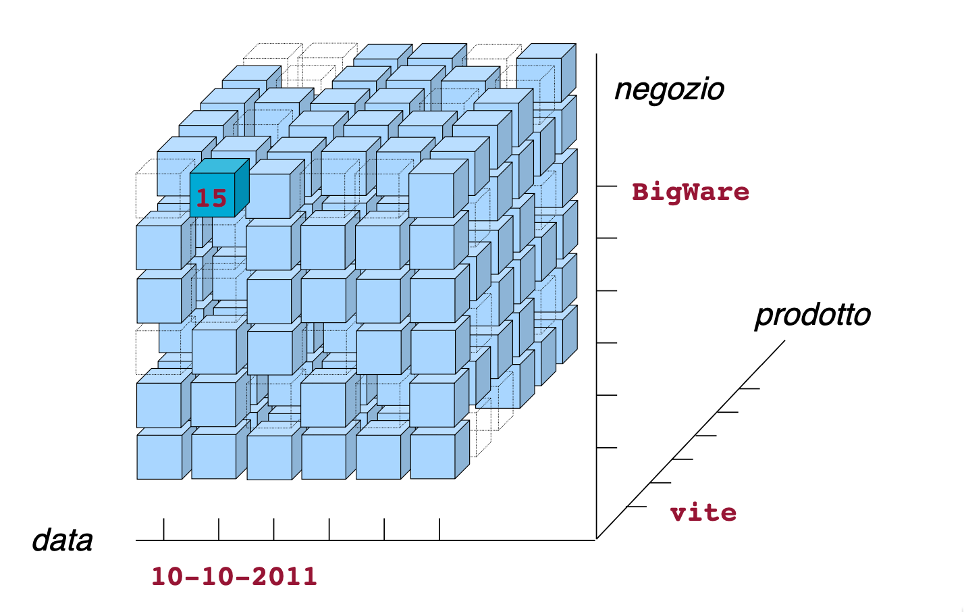
\includegraphics[width=0.7\linewidth]{img/example}
	\caption{Esempio modello multidimensionale}
	\label{fig:model}
\end{figure}
Nell'esempio in figura \ref{fig:model} sto dicendo che in quella data, nel negozio BigWare, ho venduto 15 viti. Supponendo di avere le seguenti cardinalità:
\begin{itemize}
	\item 
	Negozio : $10^{3}$
	\item 
	Data: $10^{3}$
	\item 
	Prodotto: $10^{4}$
\end{itemize}
La cardinalità massima del cubo se non ci fosse sparsità sarebbe $10^{10}$. Supponendo che un prodotto ogni 10 in un negozio e per ciascuna data resti invenduto, la cardinalità reale sarebbe di $10^{9}$. \\

Ho bisogno di tecniche per riuscire ad analizzare le informazioni in maniera più agevole, in moda da ridurne ulteriormente la mole. Nel modello multidimensionale ho due tecniche: \textbf{selezione} e \textbf{aggregazione}. L’idea della selezione, al momento del lancio di una query OLAP, è quella di concentrarsi su alcuni dati e non su altri. Nel modello multidimensionale esistono due modi differenti per fare selezione: \textbf{slicing} e \textbf{dicing}. Fare slicing significa focalizzarsi su una fetta di dati. Per fare ciò io fisso un valore da una dimensione e seleziono le celle corrispondenti a quel valore. Con il dicing io seleziono un sotto cubo rispetto al cubo di partenza specificando degli intervalli. 
\begin{figure}[H]
	\centering
	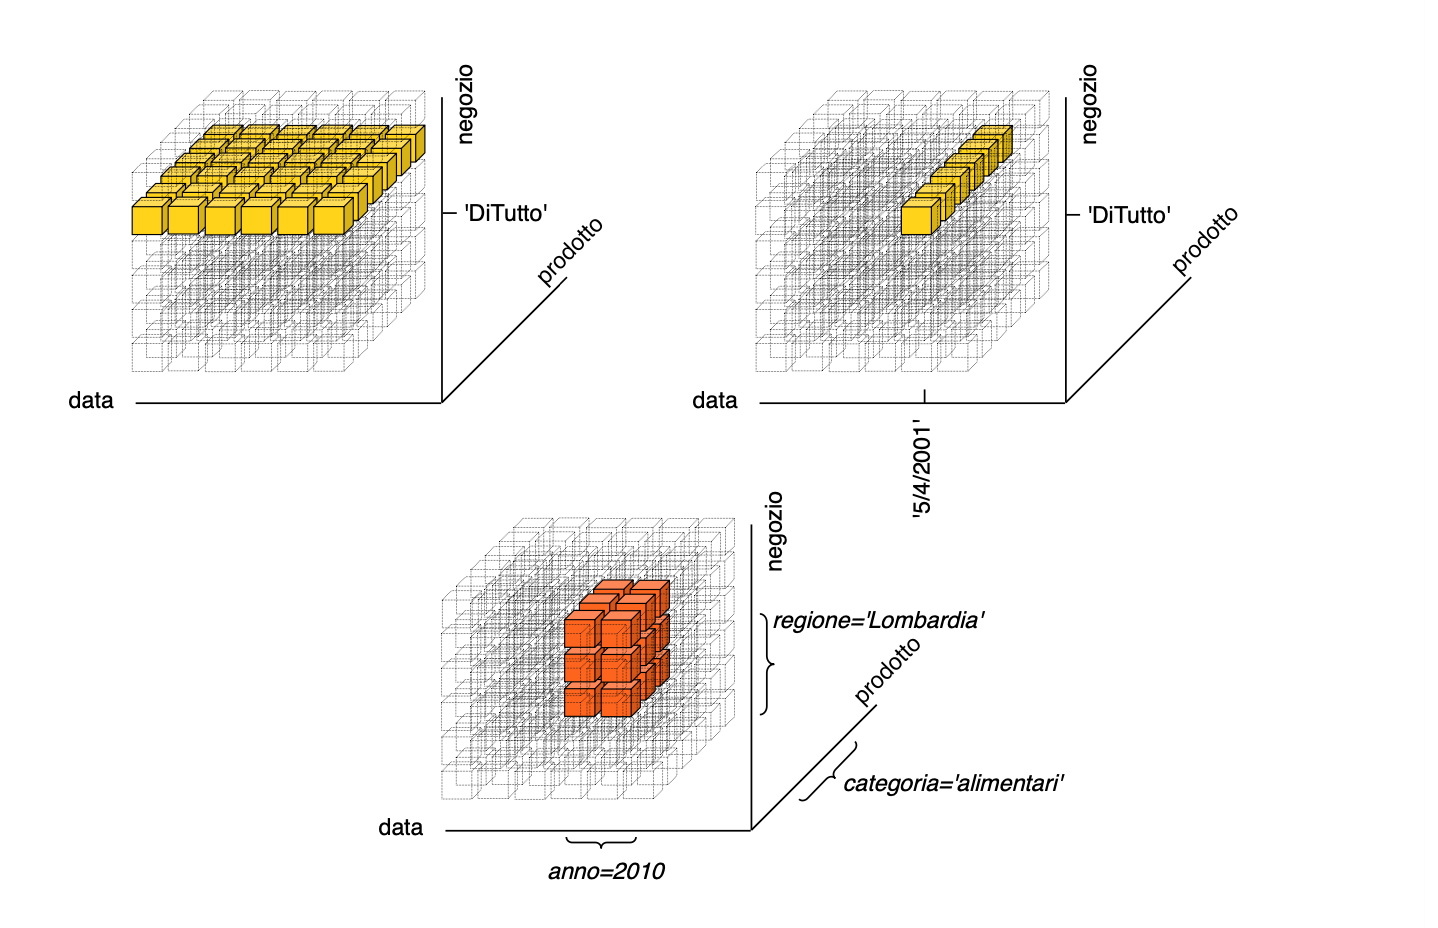
\includegraphics[width=0.5\linewidth]{img/slicing&dicing}
	\caption{Slicing and dicing}
	\label{fig:slice}
\end{figure}

Per introdurre l’\textbf{aggregazione} bisogna aggiungere il concetto di gerarchia. Una \textbf{gerarchia} è una sequenza di attributi che parte da una dimensione, nel nostro caso prodotto e negozio, collegati tra di loro da associazioni molti ad uno. 

Dato il cubo delle vendite, potrei come utente decidere che questo livello di dettaglio è troppo e vorrei analizzare il fenomeno ad un livello di granularità meno fine.
\begin{figure}[H]
	\centering
	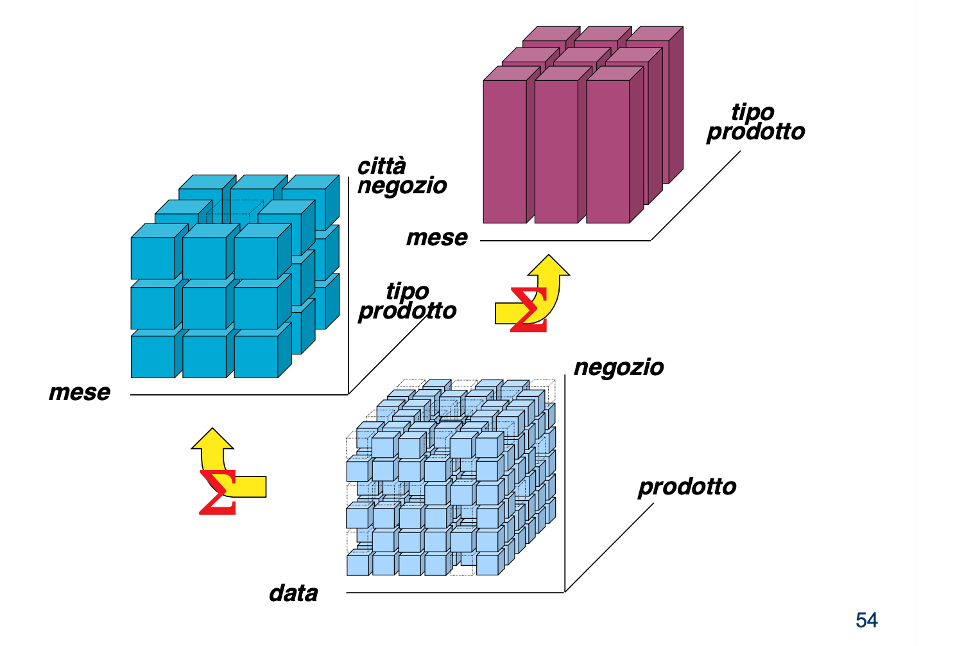
\includegraphics[width=0.6\linewidth]{img/gran}
	\caption{Aggregazione}
	\label{fig:aggregazione}
\end{figure}
\subsection{Analisi dei dati}
Esistono due approcci differenti, supportati da altrettante categorie di strumenti, all’interrogazione di un DW da parte degli utenti finali:
\begin{itemize}
	\item 
	\textbf{Reportistica}: non richiede conoscenze informatiche. La reportistica viene chiamata anche reportistica statica, per evidenziare il fatto, che quando si fa reportistica l’utente ha un ruolo passivo perché i report vengono decisi al momento del progetto e non sono modificabili interattivamente dagli utenti. Nel caso della reportistica si lavora come nel caso dell’OLTP congelando le query frequenti dentro la logica applicativa. 
	\item
	\textbf{OLAP}: ho bisogno di conoscere l’interfaccia dello strumento grafico utilizzato e avere chiaro il modello multidimensionale. Nel caso dell’OLAP l’utente non ha più un ruolo passivo ma attivo, perché sceglie quale query formulare. Gli utenti OLAP sono in grado di costruire attivamente una sessione di analisi, cioè dei percorsi di esplorazione all’interno del cubo. In questo modo pur non essendo un esperto di informatica, riesce a costruire delle sessioni di lavoro estemporanee, formulando anche delle query complesse. Una \textbf{sessione} è una sequenza di query formulate per differenza rispetto alle precedenti. Ogni passo della sessione è scandito dall’applicazione di un operatore OLAP che trasforma l’ultima interrogazione formulata in una nuova interrogazione. Il risultato delle interrogazioni è di tipo multidimensionale. 
\end{itemize}
\subsubsection{Gli operatori OLAP}
\begin{itemize}
	\item
	\textbf{Roll-Up}: parte da una certa situazione di analisi di dettaglio e  porta a fare uno zoom-out, cioè permette di aggregare il cubo. 
	\item 
	\textbf{Drill-down}: parte da un cubo grossolano e fa uno zoom-in, cioè si avvicina e scorpora i dati nelle sue componenti. Nel fare questo può anche iniettare in un cubo una dimensione che prima non c’era. 
	\item 
	\textbf{Slice-and-dice}: è un operatore di selezione che permette di focalizzarsi su un sottoinsieme di eventi del fatto o attraverso uno slicing o attraverso un dicing. La differenza è di tipo concettuale perché l’operatore è unico. 
	\item 
	\textbf{Pivoting}: è un operatore che cambia il modo per visualizzare i dati, inverte righe e colonne.
	\item 
	\textbf{Drill-across}: è un operatore di sostanza e permette di stabilire una corrispondenza tra due cubi distinti. Mette in corrispondenza una cella di un cubo con un’altra cella dell’altro cubo. Serve quando bisogna valutare una misura che ottengo applicando una formula a misure che stanno su cubi diversi. 
	\item 
	\textbf{Reportistica semi-statica}: è un approccio intermedio tra reportistica statica e OLAP. La reportistica semi-statica nasce per evitare che un cliente malaccorto lanci delle query troppo dettagliate che possano piantare il DW o aggregare con diversi operatori, ottenendo strani risultati. Si immagini che la reportistica semi-statica sia un prato in cui ci si possa muovere in alcune direzioni e non in altre; quindi, dove comunque ho dei percorsi di aggregazione.
\end{itemize}
\subsection{Implementazione Data Werahouse}
Esistono tipicamente due piattaforme tecnologiche per l’implementazione del DW:
\begin{itemize}
	\item 
	\textbf{ROLAP (Relational OLAP)}: è un’implementazione relazionale e dunque il dato multidimensionale alla fine viene implementato su un server relazionale (tabelle). Perché usare un DB relazionale se ho un modello diverso? I database relazionali sono diffusi in azienda e quindi si cerca di utilizzare ciò anche nell’ambito del DW. Devo affrontare il problema del miss match, cioè la mancata corrispondenza tra i due modelli, perché l’utente ragionerà in termini di cubi ma sotto ho delle relazioni. Per saltare questo passaggio bisogna usare delle forme particolare dei modelli relazionali per ospitare dati multidimensionali (schema a stella). Ho un problema di traduzione che viene effettuata nei due versi da un componente detto motore multidimensionale, il quale si appoggia a dei metadati per restituire una visione multidimensionale di dati relazionali. 
	\begin{figure}[H]
		\centering
		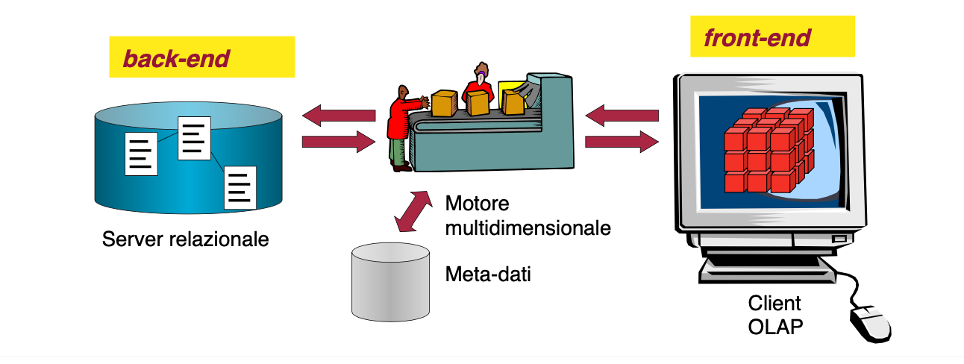
\includegraphics[width=0.7\linewidth]{img/rolap}
		\caption{ROLAP}
		\label{fig:rolap}
	\end{figure}
	Mi aspetterei potenziali problemi di prestazioni, perché per lavorare sui DB relazionali, ho bisogno di fare join che sono operazioni costose tanto più fatte su tabelle che hanno milioni di righe. Si utilizzano tecniche particolare per evitare questi problemi, come la denormalizzazione.
	\item 
	\textbf{MOLAP (Multidimensional OLAP}): basato su un database che è nativamente multidimensionale, costruito ad hoc, i dati sono allocati dentro una matrice ad accesso posizionale. Le prestazioni risultano essere ottime perché non ho bisogno di join ma al contempo ho il problema della sparsità, perché mentre in una tecnologia ROLAP nelle tabelle ho righe solo per gli eventi che si verificano, in MOLAP devo allocare tutto il cubo. Ogni piattaforma MOLAP utilizza un suo metodo per gestire la sparsità e sono poco utilizzati. 
	\item 
	\textbf{HOLAP (Hybrid OLAP)}: combinazione tra le due tecnologie in cui tipicamente i dati di dettaglio sono memorizzati su DBMS relazionale, i pre-aggregati su strutture multidimensionali proprietarie. Oppure, i sotto cubi densi sono memorizzati in forma multidimensionale, quelli sparsi in forma relazionale. 
\end{itemize}
\subsection{Qualità e Sicurezza}
In termini generali la qualità di un processo misura la sua aderenza agli obiettivi degli utenti. Nella fattispecie quando si parla di DW interessa la qualità dei dati, il quale è legata ad una buona realizzazione dell’ETL. La qualità dei dati all’interno del DW ha diversi aspetti:
\begin{itemize}
	\item 
	\textbf{Accuratezza}: c’è conformità tra il valore memorizzato e quello reale
	\item 
	\textbf{Attualità}: il dato è attuale e non obsoleto (dipende dalla frequenza dell’ETL)
	\item 
	\textbf{Completezza}: non mancano informazioni
	\item 
	\textbf{Consistenza}: sono effettivamente riuscito a superare l’eterogeneità dei dati
	\item 
	\textbf{Disponibilità}: i dati sono facilmente disponibili all’utente
	\item
	\textbf{Tracciabilità}: è possibile risalire alla fonte di ciascun dato, stabilire un collegamento tra il DB del data werahouse e il DB operazionale, in cui trovo i singoli documenti
	\item 
	\textbf{Chiarezza}: i dati sono facilmente interpretabili
\end{itemize}
Quando un progetto di DW va a regime, cioè entra in produzione,  occorre necessariamente che l’azienda attui un processo di certificazione, ossia deve individuare delle persone che siano responsabili del dato. È chiaro che questo sia un ruolo di business e non informatico, che ha dunque la sensibilità del dato. In assenza di certificazione non ho nessuna garanzia sulla qualità. 

All’interno del DW ci finiscono informazioni che sono assolutamente strategiche e che quindi non devono finire in mano ai competitor o a certi ruoli aziendali. Spesso nei DW si attua una compartimentazione dell’informazione. Ogni capo reparto vede i dati solo del suo reparto. La \textbf{sicurezza} in primis viene implementata attraverso un controllo molto stretto delle autorizzazioni, che si svolge in genere sugli strumenti di front-end OLAP. Si utilizzano meccanismi di auditing per monitorare gli accessi, il che risulta più complicato, perché siamo in presenza di aggregazione. 